\section{Portefeuilletheorie}

\textbf{Ziel}: Abwägen zwischen Ertrag und Risiko 
$\rightarrow$ Durch Erwerb verschiedener Aktien kann Risikominderung (\textbf{Diversifikation}) erreicht werden.

\textbf{Gleichgewichtstheorie (CAPM)}: Wenn alle Investoren gemäß obiger Theorie agieren, entsteht ein \enquote{fairer} Preis für ein übernommenes Risiko $\rightarrow$ CAPM liefert Zusammenhang zwischen Risiko und angemessener Rendite

\textbf{Renditen}:
\begin{itemize}
	\item \textbf{Absolute Aktienrendite} = Dividende + Kursveränderung
	\item \textbf{Aktienrendite} $r = \cfrac{\text{Dividende + Kursveränderung}}{\text{anfänglicher Vermögenswert}}$
\pagebreak
	\item \textbf{Halteperiode Rendite}: Rendite, die ein Investor erhält, wenn er eine Investition
	über $n$ Jahren hält:
	\begin{center}
		$\text{Halteperiode Rendite}=(1+r_1)\cdot(1+r_2)\cdot\ldots\cdot(1+r_n)-1$,
	\end{center}
	wobei $r_i$ die Rendite für das Jahr $i$ ist.
	\item \textbf{Geometrisch durchschnittliche Rendite}:
	\begin{center}
		 $r_g=\sqrt[n]{(1+r_1)\cdot(1+r_2)\cdot\ldots\cdot(1+r_n)}-1$
	\end{center}
	\item \textbf{Arithmetisch durchschnittliche Rendite} $r_a=\cfrac{r_1+r_2+\dots+r_n}{n}$
\end{itemize}
Für eine Historie von $T$ Renditen $R_i$ können folgende Kennzahlen bestimmt werden:
\begin{itemize}
	\item \textbf{Durchschnittliche Rendite} $\bar{R}=\cfrac{R_1+R_2+\dots+R_T}{T}$
	\item \textbf{Standardabweichung der Renditen}:
	\begin{center}
		$SD=\sqrt{VAR}=\sqrt{\cfrac{(R_1-\bar{R})^2+(R_2-\bar{R})^2+\ldots+(R_T-\bar{R})^2}{T-1}}$
	\end{center}
\end{itemize}

\textbf{Risikoprämie}: Zusätzliche Rendite über die risikolose Rendite hinaus für die Übernahme von Risiko\\

\textbf{Einzelne Wertpapiere}:
\begin{itemize}
	\item Für Wahrscheinlichkeiten $w_i$, dass eine Rendite $r_i$ eintritt, ist die
	\begin{center}
		\textbf{Erwartete Rendite} $\mu=\sum w_i\cdot r_i$
	\end{center}
	\item \textbf{Varianz} $\sigma^2=\sum (r_i-\mu)\cdot w_i$
	\item \textbf{Standardabweichung} $\sigma=\sqrt{\text{Varianz}}$
\end{itemize}
\bigskip
\textbf{Portefeuilles}: Betrachte Portefeuille mit $n$ Wertpapieren:
\begin{itemize}
	\item Sei $S_i$ der Wert der Aktie $i$ mit Einzelrendite $\tilde{r}_i$ von dem $x_i$ Stück im Portefeuille sind. Dann gilt:
	\begin{center}
		\textbf{Portefeuillerendite} $\tilde{r}_w=\sum\limits_{i=1}^n w_i\cdot\tilde{r}_i$
	\end{center}
	mit \textbf{Portefeuilleanteilen} $w_i=\cfrac{x_i\cdot S_i}{\sum\limits_{k=1}^{n}x_k\cdot S_k}$
	\item \textbf{Wert des Portefeuilles} $=\sum\limits_{k=1}^{n}x_k\cdot S_k$
	\item \textbf{Erwartete Portefeuillerendite}: $\mu_w=\E(\sum\limits_{i=1}^n w_i\cdot\tilde{r}_i)=\sum\limits_{i=1}^n w_i\cdot\mu_i$, wobei $\mu_i$ die erwartete Rendite für Aktie $i$ ist.
	\item \textbf{Varianz der Portefeuillerendite} für Portefeuille mit 2 Wertpapieren: 
	\begin{center}
		$\sigma^2_w=w_1^2\sigma_1^2+w_2^2\sigma_2^2+2w_1w_2\text{cov}_{1,2}$
	\end{center}
	mit \textbf{Kovarianz} $\text{cov}_{1,2}=\sigma_1\sigma_2\rho_{12}=\E((\tilde{r}_1-\mu_1)(\tilde{r}_2-\mu_2))$ \textit{(s. FS5/18)} und\\
	\textbf{Korrelation} $\rho_{12}\in[-1;1]$
\end{itemize}
\bigskip
\textbf{Erreichbare Rendite/Risiko-Kombinationen}:
Betrachte Einfluss des Korrelationskoeffizienten:
\begin{center}
	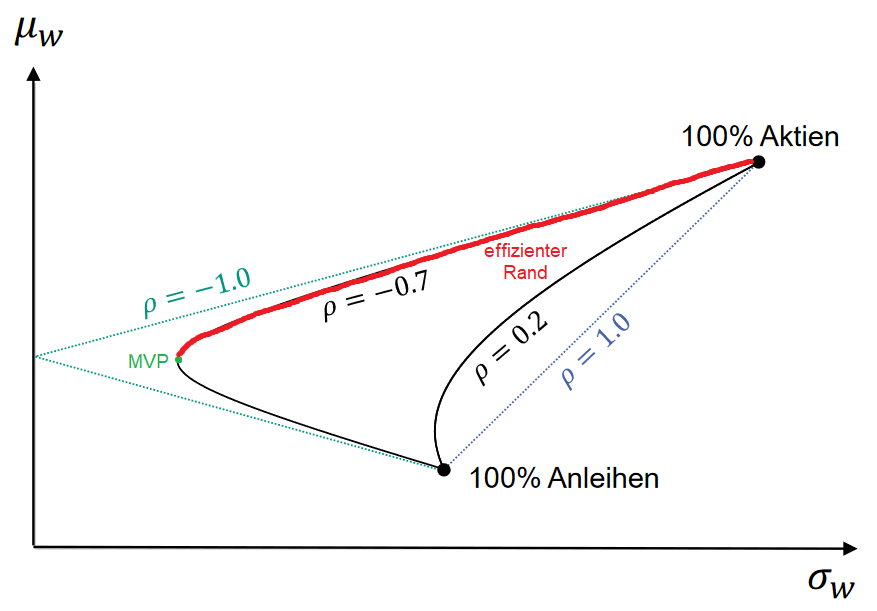
\includegraphics[width=0.6\textwidth]{images/portefeuille.png}
\end{center}
\begin{itemize}
	\item $\rho=1$: keine Risikoreduktion
	\item $\rho=-1$: vollständige Risikoeliminierung möglich
	\item Portefeuille mit kleinster Varianz heißt \textbf{Minimum Varianz Portefeuille MVP}
	\item Nur Portefeuilles oberhalb des MVP sind effizient! (\textbf{Effizienter Rand})
\end{itemize}
\bigskip
\textbf{Kombinationen mit risikolosem Wertpapier}:
\begin{center}
	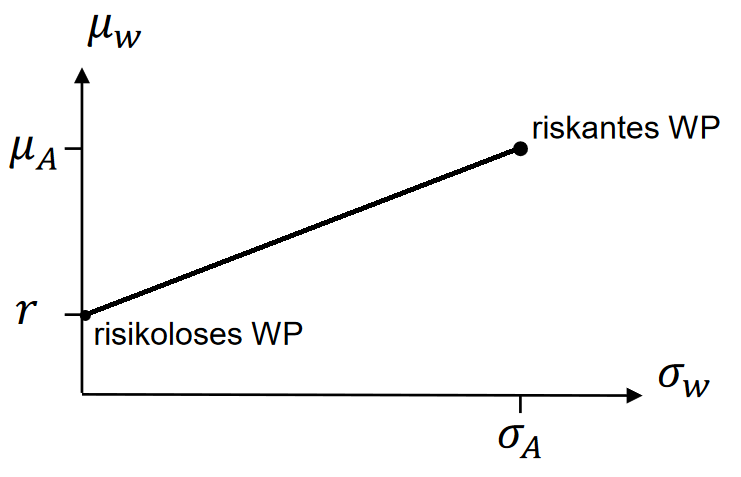
\includegraphics[width=0.5\textwidth]{images/riskfree.png}
\end{center}
Betrachte Portefeuille aus riskantem Instrument mit Anteil $w_A$ und Rendite $\tilde{r}_A$ und risikolosem Wertpapier mit Anteil $w_0$ und Rendite $r$.
\begin{itemize}
	\item \textbf{Portefeuillerendite} $\tilde{r}_w=w_A\tilde{r}_A+w_0r$
	\item \textbf{Erwartete Rendite} $\mu_w=w_A\mu_A+w_0r$
	\item \textbf{Risiko} $\sigma_w^2=w_A^2\sigma_A^2\implies\sigma_w=w_A\sigma_A\implies$ lineare Gerade s. oben
\end{itemize}
Betrachte Kombination aus risikolosem Instrument und mehreren risikobehafteten Instrumenten:
\begin{center}
	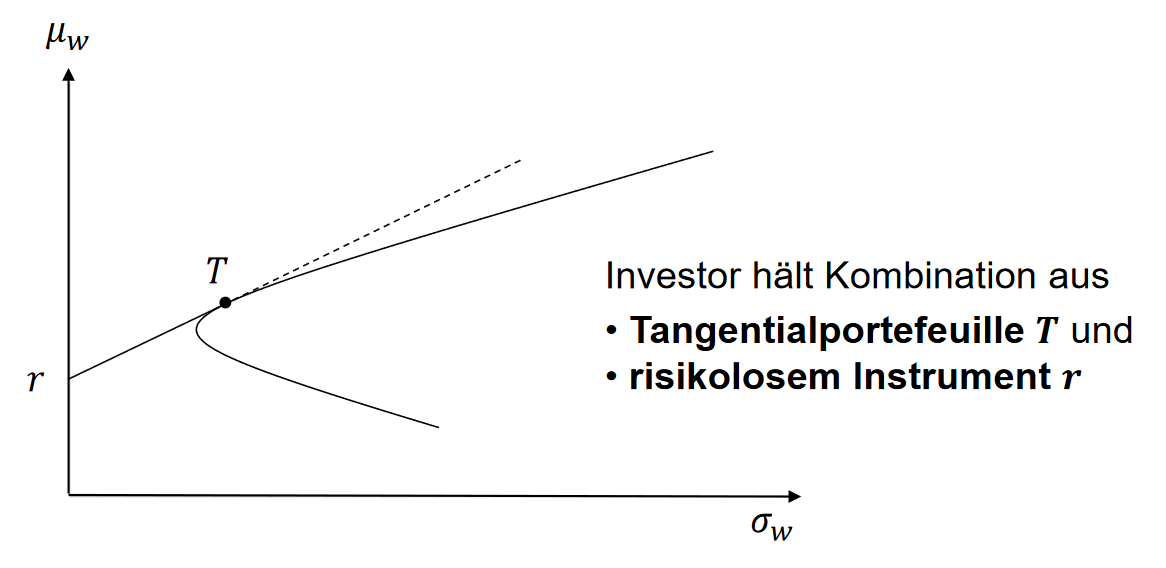
\includegraphics[width=0.65\textwidth]{images/r_and_r.png}
\end{center}
\begin{itemize}
	\item Effiziente Portefeuilles liegen auf einer Geraden: $\mu_w=r+\cfrac{\mu_T-r}{\sigma_T}\cdot\sigma_w$
	\item Gestrichelte Linie: Am Punkt $T$ wird 100\% in das Tangentialportefeuille investiert, d.h. um in den gestrichelten Bereich zu kommen, müssen Schulden aufgenommen werden
\end{itemize}
\bigskip
\textbf{Capital Asset Pricing Model (CAPM)}: Was passiert, wenn alle Investoren so wie oben agieren?
Annahmen:
\begin{itemize}
	\item Investoren sind $\mu\text{-}\sigma$-Optimierer und besitzen gleiche Erwartungen bezüglich $\mu_i,\sigma_i,\rho_{ij}$
	\item Kapitalmärkte sind friktionslos, bestehen aus $N$ verschiedenen Aktien mit festem Angebot und einem risikolosen Instrument
\end{itemize}
$\rightarrow$ Zusammensetzung des Tangentialportefeuilles für \textbf{alle Investoren identisch}\\
$\rightarrow$ Aufteilung zw. Tangentialportefeuille u. risikolosem Instrument \textbf{investorspezifisch}\\

\textbf{Vom Individualkalkül zum Gleichgewicht}:
Anpassung der Kurse heute so, dass Markträumung stattfindet \textit{(s. FS5/31-39)}, also bis Angebot=Nachfrage.\\
$\rightarrow$ Jeder Investor legt sein riskantes Vermögen in der gleichen Zusammensetzung wie das \textbf{Marktportefeuille} an.

\pagebreak
\textbf{Kapitalmarktlinie}: 
\begin{center}
	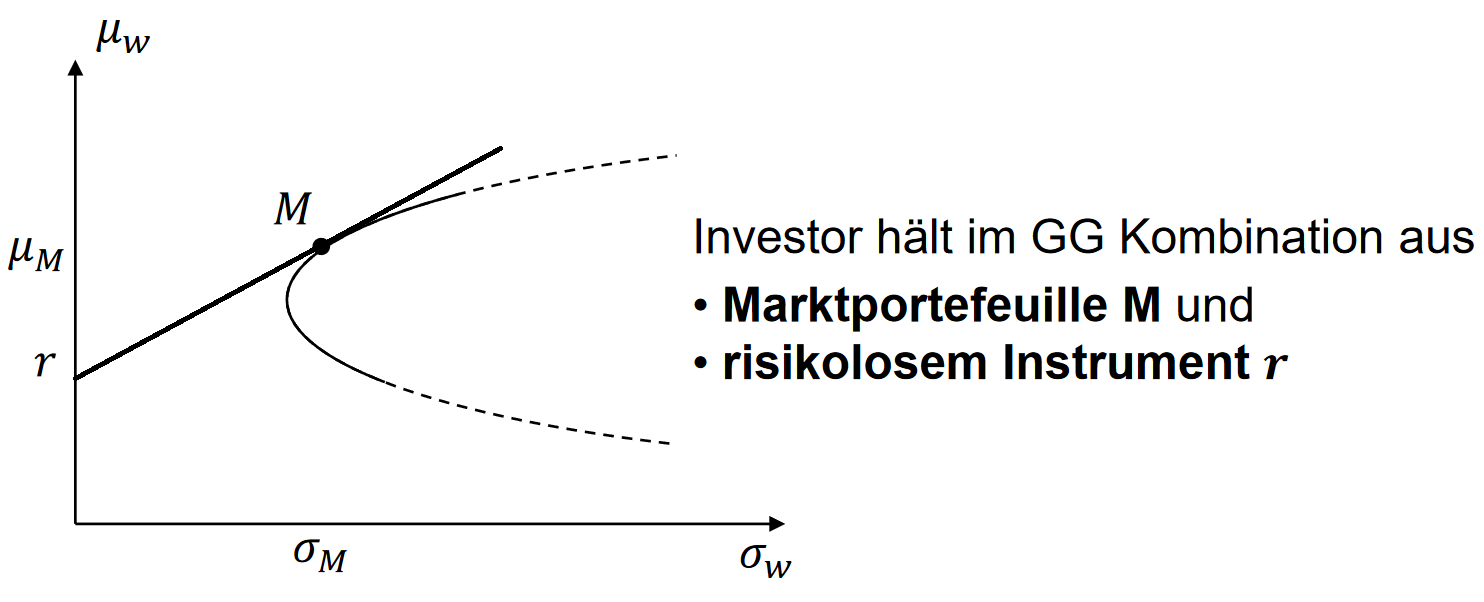
\includegraphics[width=0.65\textwidth]{images/marktpf.png}
\end{center}
\begin{itemize}
	\item Letztendlich hält jeder Investor ein kleines Abbild des Marktportefeuilles aufgrund der oben genannten Dynamik $\rightarrow$ Tangentialportefeuille ist nun das Marktportefeuille
	\item Effiziente Portefeuilles liegen auf \textbf{Kapitalmarktlinie}:
	\[
	\underbrace{\mu_w}_\text{erwartete Rendite}=
	\underbrace{r}_\text{risikolose Rendite} + 
	\underbrace{\cfrac{\mu_M-r}{\sigma_M}}_\text{Preis pro Einheit Risiko}\cdot
	\underbrace{\sigma_w}_\text{Risikomenge}
	\]
	\item $\cfrac{\mu_M-r}{\sigma_M}$ gibt an, wie viel zusätzliche Rendite im Gleichgewicht für eine Einheit\\\\ zusätzlichen Risikos zu erwarten ist
\end{itemize}
\bigskip
\textbf{Wertpapiermarktlinie}: Betrachte nun einzelne Wertpapiere, statt ganzen Portefeuilles.
Für einzelnes Wertpapier $j$ ist nur Beitrag zum Risiko des Marktportefeuilles $\text{cov}(\tilde{r}_j,\tilde{r}_M)$ relevant.
\textbf{Zentrale Beziehung zur Bewertung riskanter Wertpapiere}:
\[
\underbrace{\mu_j}_\text{erwartete Rendite}=
\underbrace{r}_\text{risikolose Rendite} + 
\underbrace{\cfrac{\mu_M-r}{\text{cov}_{M,M}}}_\text{Preis pro Einheit Risiko}\cdot
\underbrace{\text{cov}_{j,M}}_\text{Risikomenge}= r +
\underbrace{(\mu_M-r)}_\text{Marktrisikoprämie}\cdot
\beta_j
\]
mit \textbf{Beta-Faktor}: $\beta_j=\cfrac{\text{cov}_{j,M}}{\text{cov}_{M,M}}=\cfrac{\text{cov}_{j,M}}{\sigma_M^2}$.\\\\
$\rightarrow$ Varianz eines Wertpapiers als alleinige Größe nicht ausreichend für die Bewertung des Risikos. Andere Wertepapiere müssen mitbetrachtet werden $\rightarrow$ Kovarianz wichtig!
\begin{center}
	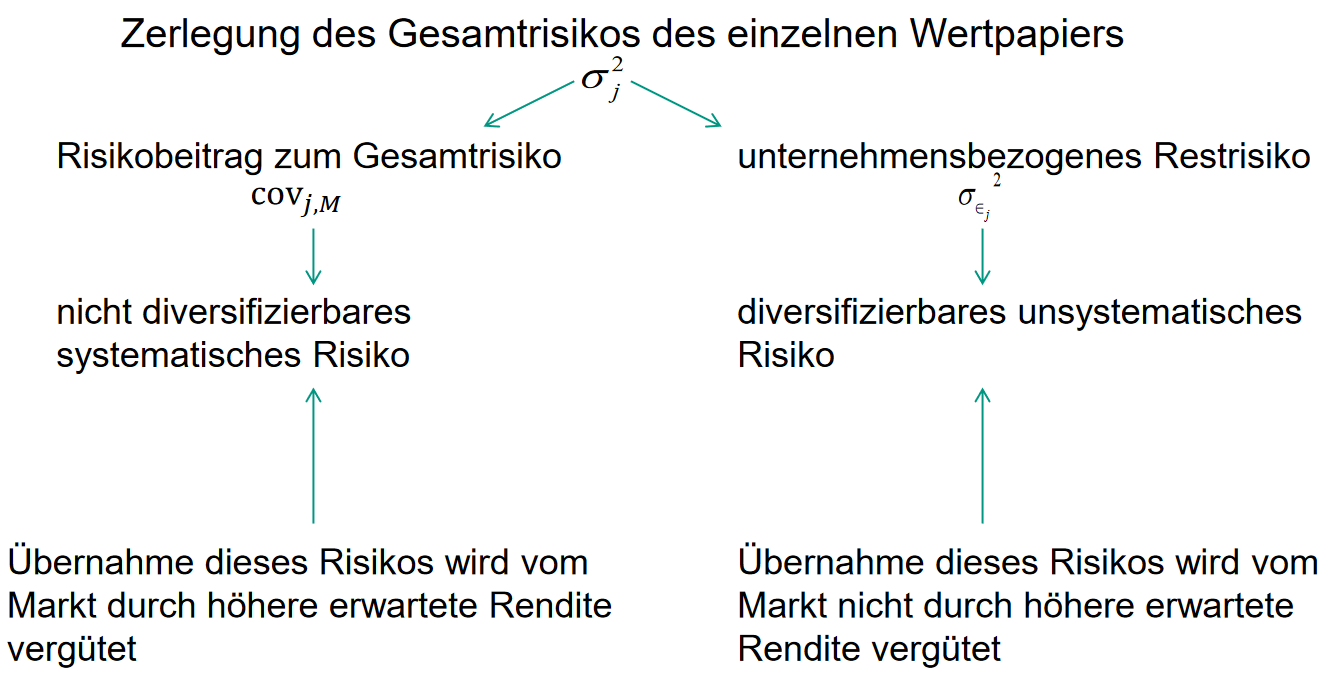
\includegraphics[width=0.8\textwidth]{images/risk-overview.png}
\end{center}
Unternehmensbezogenes Restrisiko lässt sich durch ein breites Investment weg diversifizieren, der Beitrag zum Gesamtrisiko aber nicht!